% block: partial-differential-equations-heading page:43 type:section
\subsection{{偏微分方程}}\label{sec:partial-differential-equations}
{本节通过若干偏微分方程介绍有限差分方法和有限元方法, 并将说明: 所需的解越精确, 就需要求解规模越大的线性方程组.}
% block: finite-differences-heading page:43 type:subsection
\subsubsection{{有限差分方法}}\label{subsec:finite-differences}
{本小节通过几个简单的偏微分方程介绍有限差分方法. 还将说明张量积的概念, 它便于描述偏微分方程经有限差分离散后所产生线性方程组的系数矩阵. 首先给出一些数学预备知识.}
% block: difference-preliminary-heading page:44 type:subsection
\paragraph{{预备知识}}\label{subsec:difference-preliminary}
{本小节介绍几个公式, 利用 $f(x),f(x-h)$ 和 $f(x+h)$, 在 $0<h<1$ 时近似光滑函数 $f(x)$ 在 $x$ 处的导数 $f'(x),f''(x)$. 考虑如何近似 $f'(x)$. $f(x)$ 的 Taylor 级数为}
\begin{equation}\label{eq:taylor-difference-expansion}
f(x+h)=f(x)+f'(x)h+\frac{1}{2!}f''(x)h^2+\frac{1}{3!}f'''(x)h^3+\cdots.
\end{equation}
{于是, $f'(x)$ 可写成}
\[\begin{aligned}
f'(x)&=\frac{f(x+h)-f(x)}{h}-\frac{1}{2!}f''(x)h-\frac{1}{3!}f'''(x)h^2-\cdots\\
&=\frac{f(x+h)-f(x)}{h}+O(h).
\end{aligned}\]
% block: forward-backward-differences page:44 type:ordinary-paragraph
{其中 $O(\cdot)$ 是大 O 记号. 粗略地说, 此处 $O(h)$ 表示当 $h\to0$ 时, 对适当的常数值 $c$, $-\frac{1}{2!}f''(x)h-\frac{1}{3!}f'''(x)h^2-\cdots$ 可写成 $ch$. 用递推关系}
\begin{equation}\label{eq:forward-difference}
f'(x)\approx\frac{f(x+h)-f(x)}{h}
\end{equation}
{来近似 $f'(x)$, 称为向前差分. 向前差分的精度为 $h$ 阶. 类似的近似}
\begin{equation}\label{eq:backward-difference}
f'(x)\approx\frac{f(x)-f(x-h)}{h}
\end{equation}
{称为向后差分. 向后差分的精度同样为 $h$ 阶. 为得到更精确的公式, 由 \eqref{eq:taylor-difference-expansion} 有}
\[\frac{f(x+h)-f(x-h)}{2h}=f'(x)+O(h^2),\]
{由此可得}
\begin{equation}\label{eq:central-first-difference}
f'(x)\approx\frac{f(x+h)-f(x-h)}{2h},
\end{equation}
{这称为 $f(x)$ 的一阶导数的中心差分, 精度为 $h^2$ 阶.}
% block: central-second-difference pages:44,45 type:ordinary-paragraph
{现在考虑近似二阶导数 $f''(x)$. 由 $f(x+h)$ 和 $f(x-h)$ 的 Taylor 级数 \eqref{eq:taylor-difference-expansion} 有}
\[f(x+h)-2f(x)+f(x-h)=f''(x)h^2+O(h^4).\]
{因此}
\[f''(x)=\frac{f(x+h)-2f(x)+f(x-h)}{h^2}+O(h^2).\]
{下面的近似}
\begin{equation}\label{eq:central-second-difference}
f''(x)\approx\frac{f(x+h)-2f(x)+f(x-h)}{h^2}
\end{equation}
{称为 $f(x)$ 的二阶导数的中心差分, 精度为 $h^2$ 阶.}
% block: laplace-example-heading page:45 type:subsection
\refstepcounter{applicationexample}
\paragraph{Example~\theapplicationexample\space({对称矩阵})}\label{subsec:laplace-difference}
\begingroup\makeatletter\edef\@currentlabel{\theapplicationexample}\label{ex:laplace-difference}\makeatother\endgroup
{考虑如下形式的 Laplace 方程}
\[\begin{aligned}
u_{xx}+u_{yy}&=0,&(x,y)&\in(0,1)\times(0,1),\\
u(x,y)&=g(x,y),&(x,y)&\in\Gamma,
\end{aligned}\]
{其中 $\Gamma$ 是 $(0,1)\times(0,1)$ 的边界. 具体地, 边界条件为 $u(0,y)=g(0,y)$, $u(1,y)=g(1,y)$, $u(x,0)=g(x,0)$ 和 $u(x,1)=g(x,1)$.}
{现在用中心差分 \eqref{eq:central-second-difference} 近似求解 Laplace 方程. 为此, 在 $(0,1)\times(0,1)$ 内采用含 $N\times N$ 个点的等距网格. $N=3$ ($h=1/4$) 的情形见 Fig.\ \ref{fig:laplace-grid}.}
% block: laplace-grid-figure page:45 type:figure
\begin{figure}[htbp]\centering
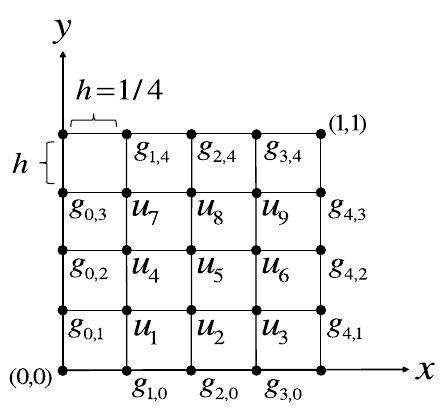
\includegraphics[width=.48\linewidth]{figures/laplace-grid.png}
\caption{{Example\ \ref{ex:laplace-difference} (Laplace 方程) 的区域网格}}\label{fig:laplace-grid}
\end{figure}
% block: five-point-discretization page:46 type:ordinary-paragraph
{下面使用 Fig.\ \ref{fig:laplace-grid} 中的网格, 说明如何得到线性方程组. 近似 $u_{xx}$ 和 $u_{yy}$ 的中心差分 \eqref{eq:central-second-difference} 为}
\begin{equation}\label{eq:laplace-xx-discretization}
u_{xx}(x,y)\approx\frac{1}{h^2}(u(x+h,y)-2u(x,y)+u(x-h,y)),
\end{equation}
\begin{equation}\label{eq:laplace-yy-discretization}
u_{yy}(x,y)\approx\frac{1}{h^2}(u(x,y+h)-2u(x,y)+u(x,y-h)).
\end{equation}
{引入简写记号 $u_{i,j}=u(x_i,y_j)$ 很方便. 于是得到下面的五点公式:}
\begin{equation}\label{eq:laplace-five-point}
u_{xx}(x_i,y_j)+u_{yy}(x_i,y_j)\approx\frac{1}{h^2}(u_{i+1,j}+u_{i-1,j}-4u_{i,j}+u_{i,j+1}+u_{i,j-1}),
\end{equation}
{其中在边界上 $u(x_i,y_j)=g(x_i,y_j)$. 令 $u_1:=u(x_1,y_1)$, $u_2:=u(x_1,y_2)$,\ldots, $u_9:=u(x_3,y_3)$, 并在边界上令 $g_{i,j}:=u(x_i,y_j)$. 于是由 Fig.\ \ref{fig:laplace-grid} 和 \eqref{eq:laplace-five-point}, 未知量 $u_1,u_2,\ldots,u_9$ 满足以下关系:}
\[\begin{aligned}
u_2+g_{0,1}-4u_1+u_4+g_{1,0}&=0,\\
u_3+u_1-4u_2+u_5+g_{2,0}&=0,\\
g_{4,1}+u_2-4u_3+u_6+g_{3,0}&=0,\\
u_5+g_{0,2}-4u_4+u_7+u_1&=0,\\
&\vdots\\
g_{4,3}+u_8-4u_9+g_{3,4}+u_6&=0.
\end{aligned}\]
% block: laplace-matrix page:46 type:equation
{相应的矩阵形式为}
\begin{equation}\label{eq:laplace-grid-system}
\underbrace{\left[\begin{array}{rrr|rrr|rrr}
-4&1&0&1&0&0&0&0&0\\1&-4&1&0&1&0&0&0&0\\0&1&-4&0&0&1&0&0&0\\\hline
1&0&0&-4&1&0&1&0&0\\0&1&0&1&-4&1&0&1&0\\0&0&1&0&1&-4&0&0&1\\\hline
0&0&0&1&0&0&-4&1&0\\0&0&0&0&1&0&1&-4&1\\0&0&0&0&0&1&0&1&-4
\end{array}\right]}_A
\underbrace{\begin{bmatrix}u_1\\u_2\\u_3\\u_4\\u_5\\u_6\\u_7\\u_8\\u_9\end{bmatrix}}_{\boldsymbol{x}}
=\underbrace{-\begin{bmatrix}g_{1,0}\\g_{2,0}\\g_{3,0}\\0\\0\\0\\0\\0\\0\end{bmatrix}
-\begin{bmatrix}0\\0\\0\\0\\0\\0\\g_{1,4}\\g_{2,4}\\g_{3,4}\end{bmatrix}
-\begin{bmatrix}g_{0,1}\\0\\0\\g_{0,2}\\0\\0\\g_{0,3}\\0\\0\end{bmatrix}
-\begin{bmatrix}0\\0\\g_{4,1}\\0\\0\\g_{4,2}\\0\\0\\g_{4,3}\end{bmatrix}}_{\boldsymbol{b}}.
\end{equation}
{求解这一线性方程组, 即可得到网格上的近似解 $u_1,\ldots,u_9$.}
% block: kronecker-definition pages:46,47 type:ordinary-paragraph
{线性方程组 \eqref{eq:laplace-grid-system} 的矩阵具有特殊的非零结构, 可利用 Kronecker 积将其改写为简单形式. 设 $A(=\{a_{ij}\})$ 和 $B$ 为矩阵. 则符号 $A\otimes B$ 称为 Kronecker 积 (或张量积), 定义为}
\begin{equation}\label{eq:kronecker-product-definition}
A\otimes B:=\begin{bmatrix}a_{11}B&\cdots&a_{1m}B\\\vdots&\ddots&\vdots\\a_{n1}B&\cdots&a_{nm}B\end{bmatrix}.
\end{equation}
{下面给出 $A,B$ 为二阶矩阵时的例子:}
\[A\otimes B=\left[\begin{array}{c|c}a_{11}B&a_{12}B\\\hline a_{21}B&a_{22}B\end{array}\right]
=\left[\begin{array}{cc|cc}
a_{11}b_{11}&a_{11}b_{12}&a_{12}b_{11}&a_{12}b_{12}\\
a_{11}b_{21}&a_{11}b_{22}&a_{12}b_{21}&a_{12}b_{22}\\\hline
a_{21}b_{11}&a_{21}b_{12}&a_{22}b_{11}&a_{22}b_{12}\\
a_{21}b_{21}&a_{21}b_{22}&a_{22}b_{21}&a_{22}b_{22}
\end{array}\right].\]
{现在令}
\[M=\begin{bmatrix}-2&1&0\\1&-2&1\\0&1&-2\end{bmatrix},\quad I=\begin{bmatrix}1&0&0\\0&1&0\\0&0&1\end{bmatrix}.\]
{则 \eqref{eq:laplace-grid-system} 中的系数矩阵 $A$ 可写成}
\begin{equation}\label{eq:laplace-kronecker-sum}
A=I\otimes M+M\otimes I.
\end{equation}
{矩阵 $A$ 的规模为 $3^2\times3^2$. 一般而言, $N\times N$ 网格产生一个 $N^2\times N^2$ 矩阵, 它可能非常大, 并且是对称的. 对称线性方程组的 Krylov 子空间方法将在 Section\ \ref{sec:hermitian-linear-systems} 中介绍. 最后, 下面列出 Kronecker 积的一些性质.}
% block: kronecker-properties pages:47,48 type:theorem
\begin{Theorem}\label{thm:kronecker-product-properties}
{Kronecker 积具有以下性质:}
\begin{enumerate}
\item {对 $A\in\mathbb{C}^{m\times n},B\in\mathbb{C}^{p\times q},C\in\mathbb{C}^{r\times s}$,}
\[(A\otimes B)\otimes C=A\otimes(B\otimes C).\]
\item {对 $A,B\in\mathbb{C}^{m\times n},C\in\mathbb{C}^{p\times q}$,}
\[(A+B)\otimes C=A\otimes C+B\otimes C.\]
\item {对 $A\in\mathbb{C}^{m\times n},B,C\in\mathbb{C}^{p\times q}$,}
\[A\otimes(B+C)=A\otimes B+A\otimes C.\]
\item {对 $c\in\mathbb{C},A\in\mathbb{C}^{m\times n},B\in\mathbb{C}^{p\times q}$,}
\[(cA)\otimes B=A\otimes(cB)=c(A\otimes B).\]
\item {对 $A\in\mathbb{C}^{m\times n},B\in\mathbb{C}^{p\times q}$,}
\[(A\otimes B)^{\mathrm H}=A^{\mathrm H}\otimes B^{\mathrm H}.\]
\item {对 $A\in\mathbb{C}^{m\times n},B\in\mathbb{C}^{p\times q},C\in\mathbb{C}^{n\times r},D\in\mathbb{C}^{q\times s}$,}
\[(A\otimes B)(C\otimes D)=(AC)\otimes(BD).\]
\end{enumerate}
\end{Theorem}
% block: kronecker-properties-proof page:48 type:proof
\begin{Proof}
{只证明第 (6) 项. $A\otimes B$ 的 $(i,k)$ 块元素为 $a_{i,k}B$, $C\otimes D$ 的 $(k,j)$ 块元素为 $c_{k,j}D$. 因此, $(A\otimes B)(C\otimes D)$ 的 $(i,j)$ 块元素为}
\[\begin{aligned}
((A\otimes B)(C\otimes D))_{i,j}&=\sum_{k=1}^n(a_{i,k}B)(c_{k,j}D)=\left(\sum_{k=1}^na_{i,k}c_{k,j}\right)BD\\
&=(AC)_{i,j}BD=((AC)\otimes(BD))_{i,j},
\end{aligned}\]
{证明完毕.}
\end{Proof}
% block: block-matrix-meaning page:48 type:ordinary-paragraph
{注意, $(i,j)$ ``块'' 元素不是标量, 而是矩阵. 例如, 考虑下列形式的二阶分块矩阵}
\[A=\begin{bmatrix}A_{11}&A_{12}\\A_{21}&A_{22}\end{bmatrix},\quad B=\begin{bmatrix}B_{11}&B_{12}\\B_{21}&B_{22}\end{bmatrix}.\]
{于是 $A$ 的 $(1,1)$ 块元素是矩阵 $A_{11}$, $B$ 的 $(1,2)$ 块元素是矩阵 $B_{12}$. 此外, 当矩阵乘法 $A_{i,j}B_{j,k}$ 有定义时, 可以把子矩阵 $A_{i,j}$ 和 $B_{i,j}$ 如同标量一样计算 $AB$. 例如, $AB$ 的 $(1,1)$ 块元素为 $A_{11}B_{11}+A_{12}B_{21}$. 由 Theorem\ \ref{thm:kronecker-product-properties} 的第 (6) 项, 下列性质成立.}
% block: kronecker-inverse page:48 type:corollary
\begin{Corollary}\label{cor:kronecker-inverse}
{设 $A$ 和 $B$ 为可逆矩阵. 则}
\[(A\otimes B)^{-1}=A^{-1}\otimes B^{-1}.\]
\end{Corollary}
% block: kronecker-inverse-proof page:48 type:proof
\begin{Proof}
{由 Theorem\ \ref{thm:kronecker-product-properties} 的第 (6) 项, 有 $(A^{-1}\otimes B^{-1})(A\otimes B)=(A^{-1}A)\otimes(B^{-1}B)=I\otimes I$, 即两个单位矩阵的 Kronecker 积. 容易看出, 单位矩阵的 Kronecker 积仍是单位矩阵.}
\end{Proof}
% block: kronecker-eigenpairs page:48 type:corollary
\begin{Corollary}\label{cor:kronecker-eigenpairs}
{设 $\boldsymbol{p}_i^{(A)}$ 和 $\boldsymbol{p}_j^{(B)}$ 分别为 $A$ 和 $B$ 的特征向量, 对应特征值为 $\lambda_i^{(A)}$ 和 $\lambda_j^{(B)}$. 则 $A\otimes B$ 的一个特征向量为 $\boldsymbol{p}_i^{(A)}\otimes\boldsymbol{p}_j^{(B)}$, 对应特征值为 $\lambda_i^{(A)}\lambda_j^{(B)}$, 即}
\[(A\otimes B)\left(\boldsymbol{p}_i^{(A)}\otimes\boldsymbol{p}_j^{(B)}\right)=\lambda_i^{(A)}\lambda_j^{(B)}\left(\boldsymbol{p}_i^{(A)}\otimes\boldsymbol{p}_j^{(B)}\right).\]
\end{Corollary}
% block: kronecker-eigenpairs-proof pages:48,49 type:proof
\begin{Proof}
{由 Theorem\ \ref{thm:kronecker-product-properties} 的第 (4) 和 (6) 项, 有}
\[(A\otimes B)\left(\boldsymbol{p}_i^{(A)}\otimes\boldsymbol{p}_j^{(B)}\right)=\left(A\boldsymbol{p}_i^{(A)}\right)\otimes\left(B\boldsymbol{p}_j^{(B)}\right)=\lambda_i\lambda_j\left(\boldsymbol{p}_i^{(A)}\otimes\boldsymbol{p}_j^{(B)}\right),\]
{证明完毕.}
\end{Proof}
% block: kronecker-sum-eigenpairs page:49 type:corollary
\begin{Corollary}\label{cor:kronecker-sum-eigenpairs}
{沿用 Corollary\ \ref{cor:kronecker-eigenpairs} 中的记号, 有}
\[(A\otimes I+I\otimes B)\left(\boldsymbol{p}_i^{(A)}\otimes\boldsymbol{p}_j^{(B)}\right)=\left(\lambda_i^{(A)}+\lambda_j^{(B)}\right)\left(\boldsymbol{p}_i^{(A)}\otimes\boldsymbol{p}_j^{(B)}\right),\]
{其中 $I$ 为单位矩阵.}
\end{Corollary}
% block: kronecker-sum-invertibility page:49 type:ordinary-paragraph
{\leavevmode\phantomsection\label{idx:chapter-02-section-01:kronecker-sum-invertibility}矩阵 $A\otimes I+I\otimes B$ 称为 Kronecker 和 (或张量和). 由 Corollary\ \ref{cor:kronecker-sum-eigenpairs} 可知, \eqref{eq:laplace-kronecker-sum} 中矩阵 $A$ 的特征向量和特征值可由 $(\boldsymbol{p}_i\otimes\boldsymbol{p}_j,\lambda_i+\lambda_j)$ 给出, 其中 $\boldsymbol{p}_i$ 和 $\lambda_i$ 为 $M$ 的第 $i$ 个特征向量和特征值. 这表明, \eqref{eq:laplace-kronecker-sum} 中的矩阵 $A$ 不可逆当且仅当存在 $i,j$ 使得 $\lambda_i=-\lambda_j$. 因而, 规模比 $A$ 小得多的矩阵 $M$ 的特征值分布决定了矩阵 $A$ 是否可逆.}
{一般而言, Kronecker 积不满足交换律, 即}
\[A\otimes B\ne B\otimes A,\]
{其中 $A\in\mathbb{C}^{m\times n}$, $B\in\mathbb{C}^{p\times q}$. 但是, 存在置换矩阵 $P_{mp}\in\mathbb{R}^{mp\times mp}$ 和 $P_{nq}\in\mathbb{R}^{nq\times nq}$ 使得}
\[P_{mp}^{\top}(A\otimes B)P_{nq}=B\otimes A.\]
{下面详细说明这一事实.}
% block: kronecker-permutation-theorem pages:49,50 type:theorem
\begin{Theorem}\label{thm:kronecker-permutation}
{设 $P_{mn}\in\mathbb{R}^{mn\times mn}$ 为如下形式的矩阵}
\begin{equation}\label{eq:kronecker-commutation-matrix}
P_{mn}=\begin{bmatrix}
(E_{11})^{\top}&(E_{12})^{\top}&\cdots&(E_{1n})^{\top}\\
(E_{21})^{\top}&(E_{22})^{\top}&\cdots&(E_{2n})^{\top}\\
\vdots&\vdots&\ddots&\vdots\\
(E_{m1})^{\top}&(E_{m2})^{\top}&\cdots&(E_{mn})^{\top}
\end{bmatrix},
\end{equation}
{其中 $E_{i,j}\in\mathbb{R}^{m\times n}$ 的 $(i,j)$ 元素为一, 其余元素为零. 则}
\[P_{mn}=P_{nm}^{\top}=P_{nm}^{-1}\]
{并且对 $A\in\mathbb{C}^{m\times n},B\in\mathbb{C}^{p\times q}$,}
\begin{equation}\label{eq:kronecker-swapping-permutation}
\underbrace{P_{mp}^{\top}}_{mp\times mp}\underbrace{(A\otimes B)}_{mp\times nq}\underbrace{P_{nq}}_{nq\times nq}=B\otimes A.
\end{equation}
{若 $A$ 和 $B$ 为方阵 (即 $m=n$, $p=q$),}
\[P_{mp}^{\top}(A\otimes B)P_{mp}=B\otimes A.\]
\end{Theorem}
% block: kronecker-permutation-proof page:50 type:proof
\begin{Proof}
{下面证明 \eqref{eq:kronecker-swapping-permutation}. \eqref{eq:kronecker-commutation-matrix} 中 $P_{m,n}$ 的 $(i,j)$ 块元素为 $E_{ij}^{\top}$, 而 $E_{ij}$ 可分解为}
\[E_{ij}=\boldsymbol{e}_i\boldsymbol{e}_j^{\top},\]
{其中 $\boldsymbol{e}_i$ 为第 $i$ 个单位向量, 即第 $i$ 个元素为一, 其余元素为零. 设 $a_{ij}$ 和 $b_{ij}$ 分别为 $A$ 和 $B$ 的 $(i,j)$ 元素. 于是, 由 \eqref{eq:kronecker-commutation-matrix}, $P_{mp}^{\top}(A\otimes B)P_{nq}$ 的 $(i,j)$ 块元素计算如下}
\[\begin{aligned}
\left(P_{mp}^{\top}(A\otimes B)P_{nq}\right)_{ij}
&=\sum_{k,\ell}E_{ki}(a_{k\ell}B)E_{\ell j}^{\top}=\sum_{k,\ell}a_{k\ell}\left(E_{ki}BE_{j\ell}\right)\\
&=\sum_{k,\ell}a_{k\ell}\left(\boldsymbol{e}_k\boldsymbol{e}_i^{\top}B\boldsymbol{e}_j\boldsymbol{e}_\ell^{\top}\right)
=\sum_{k,\ell}a_{k\ell}\left(\boldsymbol{e}_kb_{ij}\boldsymbol{e}_\ell^{\top}\right)\\
&=b_{ij}\sum_{k,\ell}a_{k\ell}\left(\boldsymbol{e}_k\boldsymbol{e}_\ell^{\top}\right)
=b_{ij}\left(\sum_{k,\ell}a_{k\ell}E_{k\ell}\right)=b_{ij}A\\
&=(B\otimes A)_{ij},
\end{aligned}\]
{证明完毕.}
\end{Proof}
% block: helmholtz-example-heading page:50 type:subsection
\refstepcounter{applicationexample}
\paragraph{Example~\theapplicationexample\space({复对称矩阵})}\label{subsec:helmholtz-difference}
\begingroup\makeatletter\edef\@currentlabel{\theapplicationexample}\label{ex:helmholtz-difference}\makeatother\endgroup
{考虑下列边值问题:}
\[\begin{aligned}
u_{xx}+u_{yy}+\sigma^2u&=0,&(x,y)&\in(0,\pi)\times(0,\pi),\\
u_x|_{x=0}&=i\sqrt{\sigma^2-\tfrac14}\cos\tfrac y2,&&\text{Neumann Condition (1)},\\
u_x|_{x=\pi}-i\sqrt{\sigma^2-\tfrac14}u|_{x=\pi}&=0,&&\text{Radiation Condition},\\
u_y|_{y=0}&=0,&&\text{Neumann Condition (2)},\\
u|_{y=\pi}&=0,&&\text{Dirichlet Condition},
\end{aligned}\]
{这一椭圆型偏微分方程称为 Helmholtz 方程, 例如见 \BookCite{19}. 为简单起见, 使用 Figs.\ \ref{fig:helmholtz-grid} 和 \ref{fig:helmholtz-ghost-grid} 所示的三乘三网格. 与上一小节的 Example\ \ref{ex:laplace-difference} 类似, 将 \eqref{eq:laplace-xx-discretization}--\eqref{eq:laplace-five-point} 应用于 Helmholtz 方程, 得}
\begin{equation}\label{eq:helmholtz-five-point}
-u_{i+1,j}-u_{i-1,j}+(4-h^2\sigma^2)u_{i,j}-u_{i,j+1}-u_{i,j-1}=0.
\end{equation}
{在 Fig.\ \ref{fig:helmholtz-ghost-grid} 给出的网格点上考虑方程 \eqref{eq:helmholtz-five-point}, 得到以下六个方程:}
% block: helmholtz-grid-figure page:51 type:figure
\begin{figure}[htbp]\centering
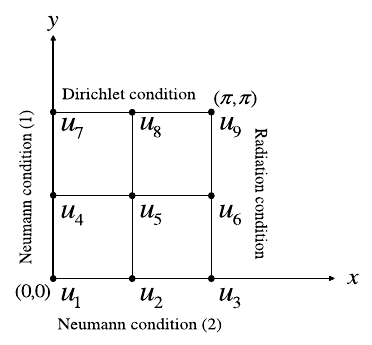
\includegraphics[width=.48\linewidth]{figures/helmholtz-grid.png}
\caption{{区域上的网格点}}\label{fig:helmholtz-grid}
\end{figure}
% block: helmholtz-ghost-grid-figure page:51 type:figure
\begin{figure}[htbp]\centering
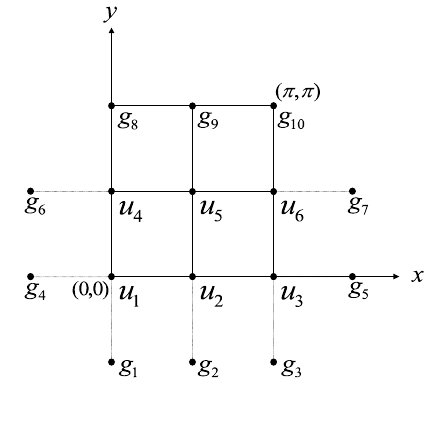
\includegraphics[width=.48\linewidth]{figures/helmholtz-ghost-grid.png}
\caption{{满足边界条件的区域网格点}}\label{fig:helmholtz-ghost-grid}
\end{figure}
% block: helmholtz-six-equations page:51 type:equation
\begin{equation}\label{eq:helmholtz-six-equations}
\left\{\begin{aligned}
-u_2-g_4-u_4-g_1+(4-h^2\sigma^2)u_1&=0,\\
-u_3-u_1-u_5-g_2+(4-h^2\sigma^2)u_2&=0,\\
-g_5-u_2-u_6-g_3+(4-h^2\sigma^2)u_3&=0,\\
-u_5-g_6-g_8-u_1+(4-h^2\sigma^2)u_4&=0,\\
-u_6-u_4-g_9-u_2+(4-h^2\sigma^2)u_5&=0,\\
-g_7-u_5-g_{10}-u_3+(4-h^2\sigma^2)u_3&=0,
\end{aligned}\right.
\end{equation}
{其中 $u_1:=u_{1,1}=u(0,0)$, $u_2:=u_{2,1}=u(h,0)$, $u_3:=u_{3,1}=u(2h,0)$, $u_4:=u_{1,2}=u(0,h)$, $u_5:=u_{2,2}=u(h,h)$, $u_6:=u_{3,2}=u(2h,h)$, 且 $h=\pi/2$. Fig.\ \ref{fig:helmholtz-ghost-grid} 中 $k=1,\ldots,10$ 对应的 $g_k$ 可通过下述四个边界条件计算: 首先, 由 Neumann Condition (2) 得}
\[\frac{u_4-g_1}{2h}=\frac{u_5-g_2}{2h}=\frac{u_6-g_3}{2h}=0,\]
{因此}
\[g_1=u_4,\quad g_2=u_5,\quad g_3=u_6.\]
{其次, 由 Neumann Condition (1) 有}
% block: helmholtz-boundary-elimination page:52 type:ordinary-paragraph
\[u_x(0,0)\approx\frac{u_2-g_4}{2h}=id\cos\left(\frac02\right),\quad
u_x(0,h)\approx\frac{u_5-g_6}{2h}=id\cos\left(\frac12\times\frac h2\right).\]
{或者等价地,}
\[g_4=u_2-2idh,\quad g_6=u_5-2idh\cos\left(\frac h4\right),\]
{其中 $d=\sqrt{\sigma^2-1/4}$. 第三, 由辐射条件得}
\[\frac{g_5-u_2}{2h}-idu_3=\frac{g_7-u_5}{2h}-idu_6=0\]
{或者等价地,}
\[g_5=u_2+2idhu_3,\quad g_7=u_5+2idhu_6.\]
{最后, 由 Dirichlet 条件可知, $g_8,g_9$ 和 $g_{10}$ 满足}
\[g_8=g_9=g_{10}=0.\]
% block: helmholtz-unscaled-system page:52 type:equation
{将 $g_1,g_2,\ldots,g_{10}$ 代入六个方程 \eqref{eq:helmholtz-six-equations}, 得到下列线性方程组:}
\begin{equation}\label{eq:helmholtz-unscaled-system}
\begin{bmatrix}
a&-2&0&-2&0&0\\-1&a&-1&0&-2&0\\0&-2&a-idh&0&0&-2\\
-1&0&0&a&-2&0\\0&-1&0&-1&a&-1\\0&0&-1&0&-2&a-idh
\end{bmatrix}
\begin{bmatrix}u_1\\u_2\\u_3\\u_4\\u_5\\u_6\end{bmatrix}
=\begin{bmatrix}f_1\\0\\0\\f_4\\0\\0\end{bmatrix},
\end{equation}
{其中 $a=\sqrt{\sigma^2-1/4}$, $f_1=-2idh$, $f_4=-2idh\cos(h/4)$. 线性方程组 \eqref{eq:helmholtz-unscaled-system} 的系数矩阵不是对称的. 对每个方程作尺度变换, 得到如下形式的对称线性方程组}
\begin{equation}\label{eq:helmholtz-symmetric-system}
\begin{bmatrix}
a/4&-1/2&0&-1/2&0&0\\-1/2&a/2&-1/2&0&-1&0\\0&-1/2&(a-idh)/4&0&0&-1/2\\
-1/2&0&0&a/2&-1&0\\0&-1&0&-1&a&-1\\0&0&-1/2&0&-1&(a-idh)/2
\end{bmatrix}
\begin{bmatrix}u_1\\u_2\\u_3\\u_4\\u_5\\u_6\end{bmatrix}
=\begin{bmatrix}f_1/4\\0\\0\\f_4/2\\0\\0\end{bmatrix}.
\end{equation}
{\eqref{eq:helmholtz-symmetric-system} 的系数矩阵不是 Hermitian 的, 但却是对称的, 即复对称的. 求解复对称线性方程组的 Krylov 子空间方法将在 Section\ \ref{sec:complex-symmetric-linear-systems} 中介绍.}
% block: nonsymmetric-example-heading page:53 type:subsection
\refstepcounter{applicationexample}
\paragraph{Example~\theapplicationexample\space({非对称矩阵})}\label{subsec:nonsymmetric-difference}
\begingroup\makeatletter\edef\@currentlabel{\theapplicationexample}\label{ex:nonsymmetric-difference}\makeatother\endgroup
{考虑下列三维偏微分方程:}
\[\begin{aligned}
[\boldsymbol{a}\cdot(\nabla*\nabla)+\boldsymbol{b}\cdot\nabla+c]u(x,y,z)&=g(x,y,z),&&\text{in }\Omega,\\
u(x,y,z)&=0,&&\text{on }\partial\Omega.
\end{aligned}\]
{这里 $\Omega$ 为立方体区域, 即 $(0,1)\times(0,1)\times(0,1)$, $\partial\Omega$ 为其边界. 符号 ``$*$'' 表示逐元素乘法. 等价地, 算子 $\boldsymbol{a}\cdot(\nabla*\nabla)+\boldsymbol{b}\cdot\nabla+c$ 可改写为}
\[a_1\frac{\partial^2}{\partial x^2}+a_2\frac{\partial^2}{\partial y^2}+a_3\frac{\partial^2}{\partial z^2}+b_1\frac{\partial}{\partial x}+b_2\frac{\partial}{\partial y}+b_3\frac{\partial}{\partial z}+c\]
{其中 $\boldsymbol{a}=[a_1,a_2,a_3]^{\top}$, $\boldsymbol{b}=[b_1,b_2,b_3]^{\top}$, $\boldsymbol{c}=[c_1,c_2,c_3]^{\top}$. 对 $u$ 的二阶导数使用中心差分 \eqref{eq:central-second-difference}, 得}
\[\begin{aligned}
a_1u_{xx}(x,y,z)&\approx\frac{a_1}{h^2}(u(x+h,y,z)-2u(x,y,z)+u(x-h,y,z)),\\
a_2u_{yy}(x,y,z)&\approx\frac{a_2}{h^2}(u(x,y+h,z)-2u(x,y,z)+u(x,y-h,z)),\\
a_3u_{zz}(x,y,z)&\approx\frac{a_3}{h^2}(u(x,y,z+h)-2u(x,y,z)+u(x,y,z-h)).
\end{aligned}\]
{类似地, 对 $u$ 的一阶导数使用中心差分 \eqref{eq:central-first-difference}, 得}
\[\begin{aligned}
b_1u_x(x,y,z)&\approx\frac{b_1}{2h}(u(x+h,y,z)-u(x-h,y,z)),\\
b_2u_y(x,y,z)&\approx\frac{b_2}{2h}(u(x,y+h,z)-u(x,y-h,z)),\\
b_3u_z(x,y,z)&\approx\frac{b_3}{2h}(u(x,y,z+h)-u(x,y,z-h)).
\end{aligned}\]
% block: nonsymmetric-grid-operator pages:53,54 type:ordinary-paragraph
{考虑一个 $(N+1)\times(N+1)\times(N+1)$ 网格, 结合上述中心差分, 得到}
\[\begin{aligned}
&[\boldsymbol{a}\cdot(\nabla*\nabla)+\boldsymbol{b}\cdot\nabla+c]u(x,y,z)\\
&\quad\approx\frac{a_1}{h^2}(u_{i+1,j,k}-2u_{i,j,k}+u_{i-1,j,k})+\frac{b_1}{2h}(u_{i+1,j,k}-u_{i-1,j,k})+cu_{i,j,k}\\
&\qquad+\frac{a_2}{h^2}(u_{i,j+1,k}-2u_{i,j,k}+u_{i,j-1,k})+\frac{b_2}{2h}(u_{i,j+1,k}-u_{i,j-1,k})\\
&\qquad+\frac{a_3}{h^2}(u_{i,j,k+1}-2u_{i,j,k}+u_{i,j,k-1})+\frac{b_3}{2h}(u_{i,j,k+1}-u_{i,j,k-1}),
\end{aligned}\]
{其中 $h=1/(N+1)$. 由于边界上 $u=0$, 沿用 Section\ \ref{subsec:laplace-difference} 中的方法, 得到}
\begin{equation}\label{eq:three-dimensional-difference-system}
(I_N\otimes I_N\otimes A+I_N\otimes B\otimes I_N+C\otimes I_N\otimes I_N)\boldsymbol{u}=\boldsymbol{g},
\end{equation}
{其中 $I_N$ 为 $N$ 行 $N$ 列的单位矩阵, $\boldsymbol{u}$ 和 $\boldsymbol{g}$ 的每个元素分别对应于 $u(x_i,y_i,z_i)$ 和 $g(x_i,y_i,z_i)$, 且}
\[\begin{aligned}
A&:=\frac{a_1}{h^2}M_1+\frac{b_1}{2h}M_2+cI_N,\\
B&:=\frac{a_2}{h^2}M_1+\frac{b_2}{2h}M_2,\\
C&:=\frac{a_3}{h^2}M_1+\frac{b_3}{2h}M_2.
\end{aligned}\]
{这里 $M_1$ 和 $M_2$ 定义为}
\[M_1:=\begin{bmatrix}-2&1&&&\\1&-2&1&&\\&\ddots&\ddots&\ddots&\\&&1&-2&1\\&&&1&-2\end{bmatrix},\quad
M_2:=\begin{bmatrix}0&1&&&\\-1&0&1&&\\&\ddots&\ddots&\ddots&\\&&-1&0&1\\&&&-1&0\end{bmatrix}.\]
{其中 $M_1$ 和 $M_2$ 为 $N$ 行 $N$ 列的 (三对角 Toeplitz) 矩阵, 矩阵中的空白位置为零.}
% block: difference-system-size page:54 type:ordinary-paragraph
{线性方程组 \eqref{eq:three-dimensional-difference-system} 的规模为 $N^3\times N^3$. 若 $N=100$, 即 $h\approx0.01$ 的等距网格, 则矩阵的阶数为一百万. 若 $N=1000$, 阶数就达到十亿! 因此, 要较好地近似求解这一偏微分方程, 就需要高效的数值求解器来求解非常大 (且稀疏) 的线性方程组.}
{当 $\boldsymbol{b}\ne0$ 时, \eqref{eq:three-dimensional-difference-system} 中的矩阵是 (实) 非对称的. 非对称 (非 Hermitian) 线性方程组的 Krylov 子空间方法将在 Section\ \ref{sec:nonhermitian-linear-systems} 中介绍.}
% block: finite-elements-heading page:54 type:subsection
\subsubsection{{有限元方法}}\label{subsec:finite-elements}
{上一小节已说明, 对 (偏) 导数作有限差分近似会得到线性递推关系, 利用这些递推关系即可建立线性方程组. 近似解对应于给定网格点上的值, 这些值就是线性方程组解向量的元素. 本小节介绍有限元方法 (下文简称 FEM), 并通过一个简单例子说明如何得到线性方程组. FEM 相对于有限差分方法的优点是: (i) 不一定需要区域上的正方形 (或矩形) 网格点, 因而它不仅适用于正方形或矩形区域, 也适用于其他各种区域; (ii) 基于泛函分析, 已有许多关于误差分析的数学结果.}
% block: poisson-domain-figure page:55 type:figure
\begin{figure}[htbp]\centering
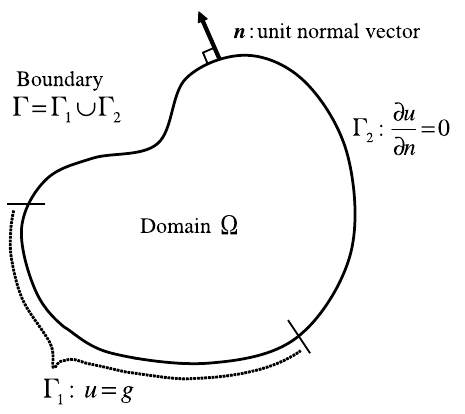
\includegraphics[width=.48\linewidth]{figures/poisson-domain.png}
\caption{{Poisson 方程 \eqref{eq:poisson-equation}--\eqref{eq:poisson-neumann} 的区域与边界}}\label{fig:poisson-domain}
\end{figure}
% block: poisson-boundary-problem page:55 type:ordinary-paragraph
{本小节考虑将 FEM 应用于下列 Poisson 方程:}
\begin{equation}\label{eq:poisson-equation}
-\Delta u(x,y)=f,\quad(x,y)\in\Omega,
\end{equation}
\begin{equation}\label{eq:poisson-dirichlet}
\cdot\ u(x,y)=g,\quad(x,y)\in\Gamma_1,\quad\text{Dirichlet Condition},
\end{equation}
\begin{equation}\label{eq:poisson-neumann}
\cdot\ \frac{\partial}{\partial n}u(x,y)=0,\quad(x,y)\in\Gamma_2,\quad\text{Neumann Condition},
\end{equation}
{其中 $\Delta:=\partial^2/\partial x^2+\partial^2/\partial y^2$. 区域以及带有边界条件的边界见 Fig.\ \ref{fig:poisson-domain}. 以下说明基于 \BookCite{118}, \BookCite{170}.}
% block: weak-form-heading page:55 type:subsection
\subsubsection{{弱形式}}\label{subsec:weak-form}
{本小节从 Poisson 方程导出称为弱形式的积分方程. 考虑将 \eqref{eq:poisson-equation} 乘以任意函数后在区域 $\Omega$ 上积分:}
\begin{equation}\label{eq:poisson-weighted-integral}
-\int_\Omega v\Delta u\,\mathrm d\Omega=\int_\Omega vf\,\mathrm d\Omega.
\end{equation}
{若能找到一个对所有 $v$ 都满足 \eqref{eq:poisson-weighted-integral} 的函数 $u$, 则 $u$ 就是 \eqref{eq:poisson-equation} 的解. FEM 试图寻找满足 \eqref{eq:poisson-weighted-integral} 的解 $u$, 而不是直接求解 \eqref{eq:poisson-equation}, 这与有限差分方法不同. 这里函数 $v$ 称为检验函数或权函数.}
% block: gauss-green-weak-form pages:55,56 type:ordinary-paragraph
{现在, 为简化数学公式, 令 $v$ 为任意光滑函数, 但在 $\Gamma_1$ 上满足 $v=0$. 对 \eqref{eq:poisson-weighted-integral} 左端应用 Gauss--Green 定理, 分部积分得}
\begin{equation}\label{eq:poisson-integration-by-parts}
\begin{aligned}
\int_\Omega v\Delta u\,\mathrm d\Omega
&=\int_\Gamma v\frac{\partial u}{\partial n}\,\mathrm d\Gamma-\int_\Omega\nabla v\cdot\nabla u\,\mathrm d\Omega\quad\text{(the Gauss--Green theorem)}\\
&=\int_{\Gamma_1}v\frac{\partial u}{\partial n}\,\mathrm d\Gamma_1+\int_{\Gamma_2}v\frac{\partial u}{\partial n}\,\mathrm d\Gamma_2-\int_\Omega\nabla v\cdot\nabla u\,\mathrm d\Omega\\
&=-\int_\Omega\nabla v\cdot\nabla u\,\mathrm d\Omega.
\end{aligned}
\end{equation}
{这里使用了 $\Gamma_1$ 上 $v=0$ 的假设以及 $\Gamma_2$ 上的 Neumann 条件 \eqref{eq:poisson-neumann}, 即 $\Gamma_2$ 上 $\frac{\partial u}{\partial n}=0$. 将 \eqref{eq:poisson-integration-by-parts} 代入 \eqref{eq:poisson-weighted-integral}, 得}
\[\int_\Omega\nabla v\cdot\nabla u\,\mathrm d\Omega=\int_\Omega vf\,\mathrm d\Omega.\]
{因此只需寻找 $u$ 使得}
\begin{equation}\label{eq:poisson-weak-form}
\iint_\Omega\left(\frac{\partial v}{\partial x}\frac{\partial u}{\partial x}+\frac{\partial v}{\partial y}\frac{\partial u}{\partial y}\right)\mathrm dx\mathrm dy=\iint_\Omega vf\,\mathrm dx\mathrm dy.
\end{equation}
{这个方程不含二阶导数, 而原方程 \eqref{eq:poisson-equation} 含有二阶导数. 换言之, \eqref{eq:poisson-weak-form} 对 $u$ 的可微性要求看来较弱. 因此, \eqref{eq:poisson-weak-form} 称为弱形式.}
% block: elementwise-weak-form page:56 type:ordinary-paragraph
{由 \eqref{eq:poisson-weak-form} 可见, 弱形式是在整个区域上积分. 现在考虑将整个区域划分成有限元 $e_i$, 即 $\Omega=\bigcup_{i=1}^n e_i$, 且当 $i\ne j$ 时 $e_i\cap e_j=\emptyset$. 于是有}
\begin{equation}\label{eq:elementwise-poisson-weak-form}
\iint_{e_i}\left(\frac{\partial v}{\partial x}\frac{\partial u}{\partial x}+\frac{\partial v}{\partial y}\frac{\partial u}{\partial y}\right)\mathrm dx\mathrm dy=\iint_{e_i}vf\,\mathrm dx\mathrm dy
\end{equation}
{其中 $i=1,2,\ldots,n$. 用三角形单元划分区域的例子见 Fig.\ \ref{fig:triangular-domain-decomposition}. 下一小节将说明如何从 \eqref{eq:elementwise-poisson-weak-form} 得到线性方程组.}
% block: element-system-derivation-heading page:56 type:subsection
\subsubsection{{线性方程组的推导}}\label{subsec:element-system-derivation}
{令 \eqref{eq:elementwise-poisson-weak-form} 中的有限元 $e_i$ 为三角形, 见 Fig.\ \ref{fig:triangular-domain-decomposition}. 三角形单元 $e_i$ 的每个节点都指定位置和编号, 三角形的节点按顺时针方向编号, 见 Fig.\ \ref{fig:triangle-node-order}. 如 Fig.\ \ref{fig:triangle-node-order} 所示, 节点 $i$ 的位置为 $(x_i,y_i)$, 其中 $i=1,2,3$.}
% block: triangular-domain-decomposition-figure page:57 type:figure
\begin{figure}[htbp]\centering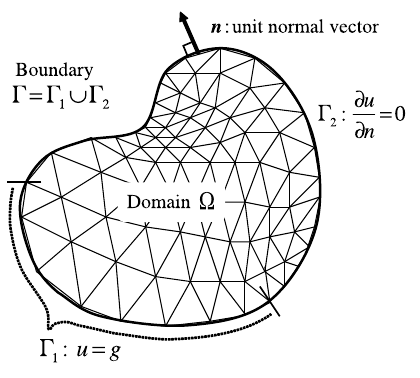
\includegraphics[width=.48\linewidth]{figures/triangular-domain-decomposition.png}
\caption{{用三角形有限元划分区域}}\label{fig:triangular-domain-decomposition}\end{figure}
% block: triangle-node-order-figure page:57 type:figure
\begin{figure}[htbp]\centering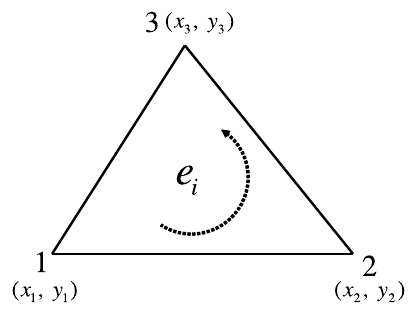
\includegraphics[width=.4\linewidth]{figures/triangle-node-order.png}
\caption{{三角形有限元的编号}}\label{fig:triangle-node-order}\end{figure}
% block: triangular-shape-functions page:57 type:ordinary-paragraph
{现在引入下列向量值函数:}
\begin{equation}\label{eq:triangle-shape-functions}
\boldsymbol{h}(x,y)=\begin{pmatrix}h_1(x,y)\\h_2(x,y)\\h_3(x,y)\end{pmatrix}
=\begin{pmatrix}1&1&1\\x_1&x_2&x_3\\y_1&y_2&y_3\end{pmatrix}^{-1}\begin{pmatrix}1\\x\\y\end{pmatrix},
\end{equation}
{并设 $\widetilde u$ 是三角形区域上解函数 $u$ 的近似函数, $\widetilde u$ 是 $x,y$ 的线性函数, 且对 $i=1,2,3$ 满足 $\widetilde u(x_i,y_i)=u_i$. 则 $\widetilde u$ 为}
\begin{equation}\label{eq:triangle-linear-interpolant}
\widetilde u=\boldsymbol{h}^{\top}\boldsymbol{u}_e=(1\ x\ y)\begin{pmatrix}1&1&1\\x_1&x_2&x_3\\y_1&y_2&y_3\end{pmatrix}^{-\top}\begin{pmatrix}u_1\\u_2\\u_3\end{pmatrix}.
\end{equation}
{等式 $\widetilde u(x_i,y_i)=u_i$ ($1\le i\le3$) 的验证留给读者作为练习.}
% block: element-gradient-integrand pages:57,58 type:ordinary-paragraph
{现在将 $\widetilde u$ 代入 \eqref{eq:elementwise-poisson-weak-form} 左侧的被积函数, 并选择与 $\widetilde u$ 具有相同形式的 $v$, 即 $v=\boldsymbol{h}^{\top}\boldsymbol{v}_e$, 其中 $\boldsymbol{v}_e:=(v_1,v_2,v_3)^{\top}$, 得}
\[\begin{aligned}
\frac{\partial v}{\partial x}\frac{\partial\widetilde u}{\partial x}+\frac{\partial v}{\partial y}\frac{\partial\widetilde u}{\partial y}
&=\frac{\partial}{\partial x}\boldsymbol{v}_e^{\top}\boldsymbol{h}\frac{\partial}{\partial x}\boldsymbol{h}^{\top}\boldsymbol{u}_e+\frac{\partial}{\partial y}\boldsymbol{v}_e^{\top}\boldsymbol{h}\frac{\partial}{\partial y}\boldsymbol{h}^{\top}\boldsymbol{u}_e\\
&=\boldsymbol{v}_e^{\top}\left(\frac{\partial}{\partial x}\boldsymbol{h}\frac{\partial}{\partial x}\boldsymbol{h}^{\top}+\frac{\partial}{\partial y}\boldsymbol{h}\frac{\partial}{\partial y}\boldsymbol{h}^{\top}\right)\boldsymbol{u}_e,
\end{aligned}\]
{其中使用了关系 $\boldsymbol{h}^{\top}\boldsymbol{v}_e=\boldsymbol{v}_e^{\top}\boldsymbol{h}$. 由 \eqref{eq:triangle-shape-functions} 可得}
\begin{equation}\label{eq:triangle-shape-x-derivative}
\boldsymbol{h}_x:=\frac{\partial\boldsymbol{h}}{\partial x}
=\begin{pmatrix}1&1&1\\x_1&x_2&x_3\\y_1&y_2&y_3\end{pmatrix}^{-1}\begin{pmatrix}0\\1\\0\end{pmatrix}
=\frac1D\begin{pmatrix}y_2-y_3\\y_3-y_1\\y_1-y_2\end{pmatrix}:=\begin{pmatrix}b_1\\b_2\\b_3\end{pmatrix},
\end{equation}
\begin{equation}\label{eq:triangle-shape-y-derivative}
\boldsymbol{h}_y:=\frac{\partial\boldsymbol{h}}{\partial y}
=\begin{pmatrix}1&1&1\\x_1&x_2&x_3\\y_1&y_2&y_3\end{pmatrix}^{-1}\begin{pmatrix}0\\0\\1\end{pmatrix}
=\frac1D\begin{pmatrix}x_3-x_2\\x_1-x_3\\x_2-x_1\end{pmatrix}:=\begin{pmatrix}c_1\\c_2\\c_3\end{pmatrix},
\end{equation}
{其中 $D$ 定义为}
\[D:=\det\begin{pmatrix}1&1&1\\x_1&x_2&x_3\\y_1&y_2&y_3\end{pmatrix}.\]
% block: element-stiffness-matrix page:58 type:ordinary-paragraph
{其中 $D$ 是三角形面积的两倍. 由于 $\boldsymbol{h}_x$ 和 $\boldsymbol{h}_y$ 不依赖于 $x,y$, \eqref{eq:elementwise-poisson-weak-form} 的左端计算如下:}
\[\begin{aligned}
\iint_{e_i}\left(\frac{\partial v}{\partial x}\frac{\partial\widetilde u}{\partial x}+\frac{\partial v}{\partial y}\frac{\partial\widetilde u}{\partial y}\right)\mathrm dx\mathrm dy
&=\boldsymbol{v}_e^{\top}(\boldsymbol{h}_x\boldsymbol{h}_x^{\top}+\boldsymbol{h}_y\boldsymbol{h}_y^{\top})\boldsymbol{u}_e\iint_{e_i}\mathrm dx\mathrm dy\\
&=\boldsymbol{v}_e^{\top}\frac{(\boldsymbol{h}_x\boldsymbol{h}_x^{\top}+\boldsymbol{h}_y\boldsymbol{h}_y^{\top})D}{2}\boldsymbol{u}_e\\
&=\boldsymbol{v}_e^{\top}A_e\boldsymbol{u}_e.
\end{aligned}\]
{这里 $\iint_{e_i}\mathrm dx\mathrm dy$ 为三角形 $e_i$ 的面积, 即 $D/2$. 矩阵 $A_e$ 是一个 $3\times3$ 对称矩阵, 其 $(i,j)$ 元素 $a_{ij}^{(e)}$ 由下式给出}
\begin{equation}\label{eq:element-stiffness-entry}
a_{ij}^{(e)}=\frac D2(b_ib_j+c_ic_j),
\end{equation}
{这是由 \eqref{eq:triangle-shape-x-derivative} 和 \eqref{eq:triangle-shape-y-derivative} 得到的. \eqref{eq:elementwise-poisson-weak-form} 的右端可写成}
\begin{equation}\label{eq:element-load-vector}
\boldsymbol{f}_e:=\begin{pmatrix}f_1^{(e)}\\f_2^{(e)}\\f_3^{(e)}\end{pmatrix}
=\begin{pmatrix}\iint_{e_i}f_0h_1\,\mathrm dx\mathrm dy\\\iint_{e_i}f_0h_2\,\mathrm dx\mathrm dy\\\iint_{e_i}f_0h_3\,\mathrm dx\mathrm dy\end{pmatrix}
=\frac{f_0D}{6}\begin{pmatrix}1\\1\\1\end{pmatrix},
\end{equation}
{其中为简单起见, 使用了 $f(x,y)=f_0$ (常函数). 于是有}
\[\iint_{e_i}vf\,\mathrm dx\mathrm dy=\boldsymbol{v}_e^{\top}\boldsymbol{f}_e.\]
% block: element-assembly-principle page:59 type:ordinary-paragraph
{计算 \eqref{eq:element-load-vector} 的右端时, 被积函数 $h_i$ ($1\le i\le3$) 为高为 1, 底面积为 $D/2$ 的三棱锥. 因此三棱锥的体积为 $(D/2)\cdot1\cdot1/3=D/6$. 由此, \eqref{eq:elementwise-poisson-weak-form} 的左端和右端分别近似为}
\begin{equation}\label{eq:element-weak-matrix-pair}
\boldsymbol{v}_e^{\top}A_e\boldsymbol{u}_e,\quad\boldsymbol{v}_e^{\top}\boldsymbol{f}_e.
\end{equation}
{上述过程是对小区域 $e_i$ 推导 \eqref{eq:element-weak-matrix-pair}. 将所有 $e_i$ 的线性方程组与边界条件一同考虑, 就得到大型线性方程组. 求解该大型线性方程组, 即可得到各节点上的近似解 $u_i$. 下一小节将说明如何得到大型线性方程组.}
% block: finite-element-example-heading page:59 type:subsection
\subsubsection{Example}\label{subsec:finite-element-example}
{作为上一小节的例子, 考虑 Fig.\ \ref{fig:square-poisson-domain} 中 $(0,1)\times(0,1)$ 正方形区域 $\Omega$ 上的 Poisson 方程 \eqref{eq:poisson-equation}, 并说明如何得到线性方程组.}
{首先把 Fig.\ \ref{fig:square-poisson-domain} 中的正方形区域划分成 Fig.\ \ref{fig:eight-triangle-mesh} 中的八个三角形. 接着, 对 Fig.\ \ref{fig:eight-triangle-mesh} 中每个三角形单元的 $A_e$ 和 $\boldsymbol{f}_e$ 计算 \eqref{eq:element-weak-matrix-pair}, 最后将所有信息组合起来, 得到线性方程组.}
{下面对 $A_e$ 和 $\boldsymbol{f}_e$ 计算 \eqref{eq:element-weak-matrix-pair}. 由 Fig.\ \ref{fig:eight-triangle-mesh} 可见, 有两类三角形: $e_1^{\mathrm I},e_3^{\mathrm I},e_5^{\mathrm I},e_7^{\mathrm I}$ 为 I 型, $e_2^{\mathrm {II}},e_4^{\mathrm {II}},e_6^{\mathrm {II}},e_8^{\mathrm {II}}$ 为 II 型, 从而产生与 \eqref{eq:laplace-five-point} 对应的两类线性方程组. 两类三角形的详情见 Fig.\ \ref{fig:two-triangle-types}.}
% block: square-poisson-domain-figure page:59 type:figure
\begin{figure}[htbp]\centering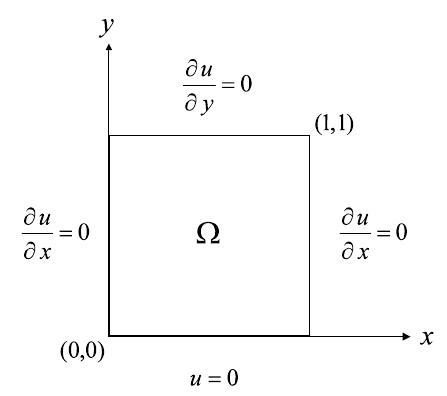
\includegraphics[width=.48\linewidth]{figures/square-poisson-domain.png}
\caption{{正方形区域 $(0,1)\times(0,1)$}}\label{fig:square-poisson-domain}\end{figure}
% block: eight-triangle-mesh-figure page:60 type:figure
\begin{figure}[htbp]\centering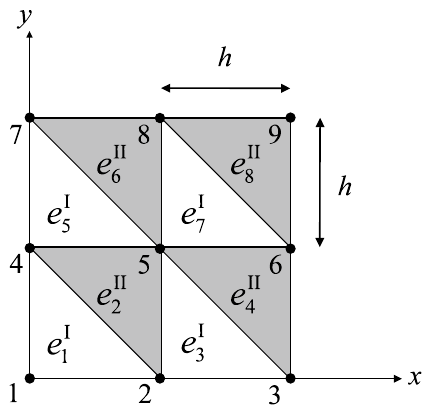
\includegraphics[width=.48\linewidth]{figures/eight-triangle-mesh.png}
\caption{{三角形网格}}\label{fig:eight-triangle-mesh}\end{figure}
% block: two-triangle-types-figure page:60 type:figure
\begin{figure}[htbp]\centering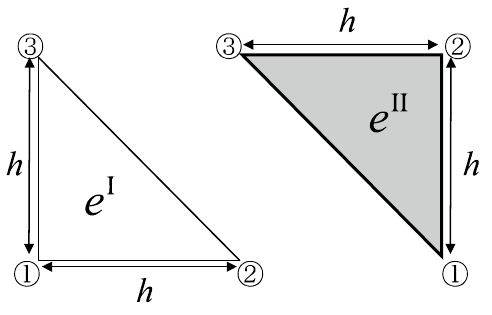
\includegraphics[width=.55\linewidth]{figures/two-triangle-types.png}
\caption{{两类三角形}}\label{fig:two-triangle-types}\end{figure}
% block: type-one-element pages:59,60 type:ordinary-paragraph
{对 I 型三角形, 由 \eqref{eq:triangle-shape-x-derivative}, \eqref{eq:triangle-shape-y-derivative}, 并回顾 $D$ 为三角形面积的两倍 (即 $D=h^2$), 有}
\[\begin{pmatrix}b_1\\b_2\\b_3\end{pmatrix}=\frac1{h^2}\begin{pmatrix}-h\\h\\0\end{pmatrix},\quad
\begin{pmatrix}c_1\\c_2\\c_3\end{pmatrix}=\frac1{h^2}\begin{pmatrix}-h\\0\\h\end{pmatrix}.\]
{于是由 \eqref{eq:element-stiffness-entry} 和 \eqref{eq:element-load-vector} 得}
\begin{equation}\label{eq:type-one-element-matrix}
A_{e^{\mathrm I}}=\frac12\begin{pmatrix}2&-1&-1\\-1&1&0\\-1&0&1\end{pmatrix},\quad
\boldsymbol{f}_{e^{\mathrm I}}=\frac{f_0h^2}{6}\begin{pmatrix}1\\1\\1\end{pmatrix},
\end{equation}
{它们对应于 \eqref{eq:element-weak-matrix-pair}. 类似地, 对 II 型三角形有}
\[\begin{pmatrix}b_1\\b_2\\b_3\end{pmatrix}=\frac1{h^2}\begin{pmatrix}0\\h\\-h\end{pmatrix},\quad
\begin{pmatrix}c_1\\c_2\\c_3\end{pmatrix}=\frac1{h^2}\begin{pmatrix}-h\\h\\0\end{pmatrix},\]
{因而}
\begin{equation}\label{eq:type-two-element-matrix}
A_{e^{\mathrm {II}}}=\frac12\begin{pmatrix}1&-1&0\\-1&2&-1\\0&-1&1\end{pmatrix},\quad
\boldsymbol{f}_{e^{\mathrm {II}}}=\frac{f_0h^2}{6}\begin{pmatrix}1\\1\\1\end{pmatrix}.
\end{equation}
% block: local-global-node-table page:61 type:table
\begin{table}[htbp]\centering
\caption{{局部节点编号与全局节点编号的关系.}}\label{tab:local-global-node-numbers}
\begin{tabular}{c|cccccccc}\hline
{单元}&$e_1^{\mathrm I}$&$e_2^{\mathrm {II}}$&$e_3^{\mathrm I}$&$e_4^{\mathrm {II}}$&$e_5^{\mathrm I}$&$e_6^{\mathrm {II}}$&$e_7^{\mathrm I}$&$e_8^{\mathrm {II}}$\\\hline
\shortstack{{三角形单元}\\{节点编号}}&\multicolumn{8}{c}{{整体节点编号}}\\\hline
1&1&2&2&3&4&5&5&6\\2&2&5&3&6&5&8&6&9\\3&4&4&5&5&7&7&8&8\\\hline
\end{tabular}\end{table}
% block: first-element-assembly page:61 type:ordinary-paragraph
{下面说明如何组合所有信息来得到线性方程组. 为此, 需要将 Fig.\ \ref{fig:eight-triangle-mesh} 中的全局节点编号 1--9 与 Fig.\ \ref{fig:two-triangle-types} 中的局部节点编号 1, 2, 3 对应起来, 所得结果见 Table\ \ref{tab:local-global-node-numbers}. 最后按如下方式导出线性方程组. 首先考虑三角形单元 $e_1^{\mathrm I}$. 由 \eqref{eq:type-one-element-matrix} 和 Table\ \ref{tab:local-global-node-numbers} 有}
\[A_{e_1^{\mathrm I}}=\frac12\begin{array}{c@{}c}
\begin{pmatrix}2&-1&-1\\-1&1&0\\-1&0&1\end{pmatrix}&\begin{matrix}1\\2\\4\end{matrix}\\
\begin{matrix}1&2&4\end{matrix}&\end{array},\quad
\boldsymbol{f}_{e^{\mathrm I}}=\frac{f_0h^2}{6}\begin{array}{c@{}c}\begin{pmatrix}1\\1\\1\end{pmatrix}&\begin{matrix}1\\2\\4\end{matrix}\end{array}\]
{利用这些信息, 构造如下矩阵和右端项:}
\[\frac12\begin{array}{c@{}c}
\begin{pmatrix}
\mathbf2&\mathbf{-1}&0&\mathbf{-1}&0&0&0&0&0\\
\mathbf{-1}&\mathbf1&0&\mathbf0&0&0&0&0&0\\
0&0&0&0&0&0&0&0&0\\
\mathbf{-1}&\mathbf0&0&\mathbf1&0&0&0&0&0\\
0&0&0&0&0&0&0&0&0\\0&0&0&0&0&0&0&0&0\\0&0&0&0&0&0&0&0&0\\0&0&0&0&0&0&0&0&0\\0&0&0&0&0&0&0&0&0
\end{pmatrix}&\begin{matrix}\mathbf1\\\mathbf2\\3\\\mathbf4\\5\\6\\7\\8\\9\end{matrix}\\
\begin{matrix}\mathbf1&\mathbf2&3&\mathbf4&5&6&7&8&9\end{matrix}&
\end{array},\quad\frac{f_0h^2}{6}\begin{array}{c@{}c}
\begin{pmatrix}\mathbf1\\\mathbf1\\0\\\mathbf1\\0\\0\\0\\0\\0\end{pmatrix}&\begin{matrix}\mathbf1\\\mathbf2\\3\\\mathbf4\\5\\6\\7\\8\\9\end{matrix}
\end{array}\]
{作为线性方程组的矩阵和右端项. 接着考虑三角形单元 $e_2^{\mathrm {II}}$. 由 \eqref{eq:type-two-element-matrix} 和 Table\ \ref{tab:local-global-node-numbers} 有}
\[A_{e_2^{\mathrm {II}}}=\frac12\begin{array}{c@{}c}
\begin{pmatrix}1&-1&0\\-1&2&-1\\0&-1&1\end{pmatrix}&\begin{matrix}2\\5\\4\end{matrix}\\
\begin{matrix}2&5&4\end{matrix}&\end{array},\quad
\boldsymbol{f}_{e^{\mathrm {II}}}=\frac{f_0h^2}{6}\begin{array}{c@{}c}\begin{pmatrix}1\\1\\1\end{pmatrix}&\begin{matrix}2\\5\\4\end{matrix}\end{array}\]
% block: second-element-assembly page:62 type:ordinary-paragraph
{将这些信息加到前述矩阵和右端项上, 得到}
\[\frac12\begin{array}{c@{}c}
\begin{pmatrix}
2&-1&0&-1&0&0&0&0&0\\
-1&\mathbf2&0&\mathbf0&\mathbf{-1}&0&0&0&0\\
0&0&0&0&0&0&0&0&0\\
-1&\mathbf0&0&\mathbf2&\mathbf{-1}&0&0&0&0\\
0&\mathbf{-1}&0&\mathbf{-1}&\mathbf2&0&0&0&0\\
0&0&0&0&0&0&0&0&0\\0&0&0&0&0&0&0&0&0\\0&0&0&0&0&0&0&0&0\\0&0&0&0&0&0&0&0&0
\end{pmatrix}&\begin{matrix}1\\\mathbf2\\3\\\mathbf4\\\mathbf5\\6\\7\\8\\9\end{matrix}\\
\begin{matrix}1&\mathbf2&3&\mathbf4&\mathbf5&6&7&8&9\end{matrix}&
\end{array},\quad\frac{f_0h^2}{6}\begin{array}{c@{}c}
\begin{pmatrix}1\\\mathbf2\\0\\\mathbf2\\\mathbf1\\0\\0\\0\\0\end{pmatrix}&\begin{matrix}1\\\mathbf2\\3\\\mathbf4\\\mathbf5\\6\\7\\8\\9\end{matrix}
\end{array}\]
{对其余单元 $e_3^{\mathrm I},e_4^{\mathrm {II}},\ldots,e_8^{\mathrm {II}}$ 作类似处理, 最终得到}
\[\frac12\begin{pmatrix}
2&-1&0&-1&0&0&0&0&0\\-1&4&-1&0&-2&0&0&0&0\\0&-1&2&0&0&-1&0&0&0\\
-1&0&0&4&-2&0&-1&0&0\\0&-2&0&-2&8&-2&0&-2&0\\0&0&-1&0&-2&4&0&0&-1\\
0&0&0&-1&0&0&2&-1&0\\0&0&0&0&-2&0&-1&4&-1\\0&0&0&0&0&-1&0&-1&2
\end{pmatrix}\begin{pmatrix}u_1\\u_2\\u_3\\u_4\\u_5\\u_6\\u_7\\u_8\\u_9\end{pmatrix}
=\frac{f_0h^2}{6}\begin{pmatrix}1\\3\\2\\3\\6\\3\\2\\3\\1\end{pmatrix}.\]
% block: finite-element-dirichlet-elimination page:62 type:ordinary-paragraph
{这一线性方程组尚未包含 Dirichlet 条件 (对 $x\in[0,1]$, 有 $u(x,0)=0$) 的信息. 由 Figs.\ \ref{fig:square-poisson-domain} 和 \ref{fig:eight-triangle-mesh} 可知, 满足 Dirichlet 条件要求}
\[u_1=u_2=u_3=0.\]
{因此, 从线性方程组中删去前三行, 并将 $u_1=u_2=u_3=0$ 代入所得线性方程组, 得到:}
\begin{equation}\label{eq:finite-element-square-system}
\frac12\begin{pmatrix}
4&-2&0&-1&0&0\\-2&8&-2&0&-2&0\\0&-2&4&0&0&-1\\
-1&0&0&2&-1&0\\0&-2&0&-1&4&-1\\0&0&-1&0&-1&2
\end{pmatrix}\begin{pmatrix}u_4\\u_5\\u_6\\u_7\\u_8\\u_9\end{pmatrix}
=\frac{f_0h^2}{6}\begin{pmatrix}3\\6\\3\\2\\3\\1\end{pmatrix}.
\end{equation}
{求解线性方程组, 即可得到 $u_4,u_5,\ldots,u_9$.}
% block: finite-element-exact-comparison page:63 type:ordinary-paragraph
{最后比较近似解与精确解. Poisson 方程的精确解为 $u(x,y)=f_0y-\frac12f_0y^2$. 当 $f_0=1$ 时, 精确解的 $u_4,u_5,u_6$ 的值为 0.375, $u_7,u_8,u_9$ 的值为 0.5. 取 $f_0=1$, $h=\frac12$ 求解线性方程组 \eqref{eq:finite-element-square-system}, 得 $u_4\approx0.381,u_5\approx0.375,u_6\approx0.369$ 和 $u_7\approx0.524,u_8\approx0.500,u_9\approx0.476$.}
{若需要更精确的近似解, 应增加节点数. 由上述推导可见, 线性方程组的规模与整体节点数几乎相同.}
